\subsubsection{UI}%
\label{sec:user-interface}
In the beginning, an app \gls{ui} was initially thought out and made a first test design.
When the user opens the program, the image of the RFCAR appears along with a built-in set of features. It is then explained the vehicle purpose as a navigation tool through inhospitable environments.
%
Following that, on the top left corner, there's a button that when pressed it redirects to the main app activity allowing first-person vision on the controlled car just like a simulated car game, only this time in a real-life scenario. Some statistics, such as the transport position and its velocity, appear in front of full-screen video capture.
%
From that point on, one can also choose to see the map and possibly the route traced along with some more detailed statistics of the remote control car. This first \gls{ui} idea is depicted in figure \ref{fig:first-ui-idea}. Later, some \gls{ui} tests were made in terms of app functionality. One had to make sure the application behaved properly without crashing when, for example, the user intends to rotate the screen. Some activities' (app screens) orientation was fixed to ensure correct behaviour. The ones where that wasn't an issue, a version for landscape was created and tested (figure \ref{fig:orientation-test}). 
%
\begin{figure}[!ht]
\centering
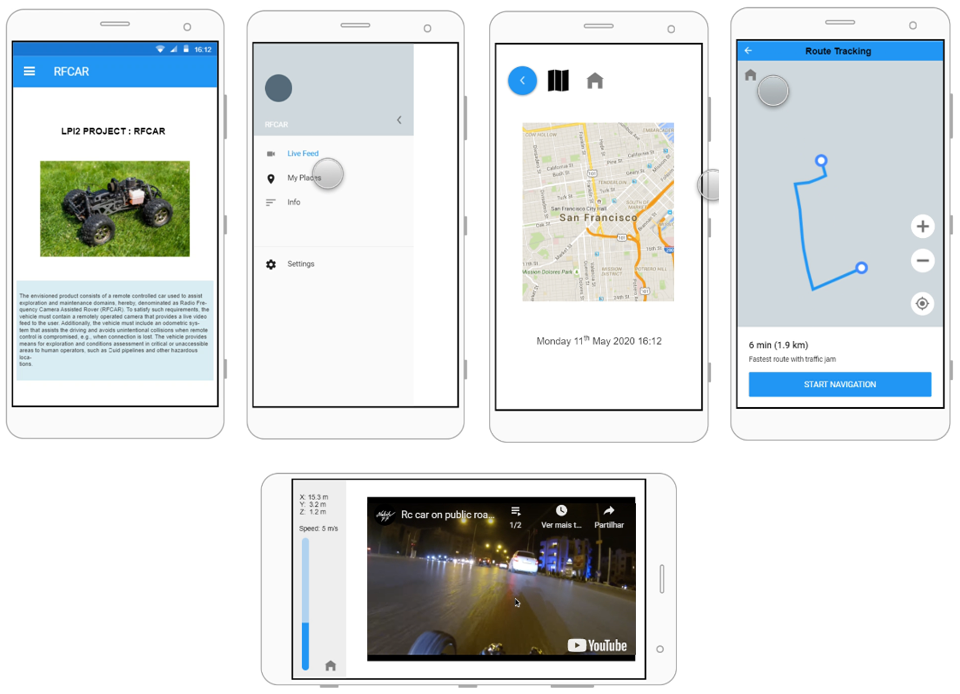
\includegraphics[width=0.8\textwidth]{img/Initial-app-idea.png}
\caption{\label{fig:first-ui-idea}First UI idea}
\end{figure}
%
\begin{figure}[!ht]
\centering
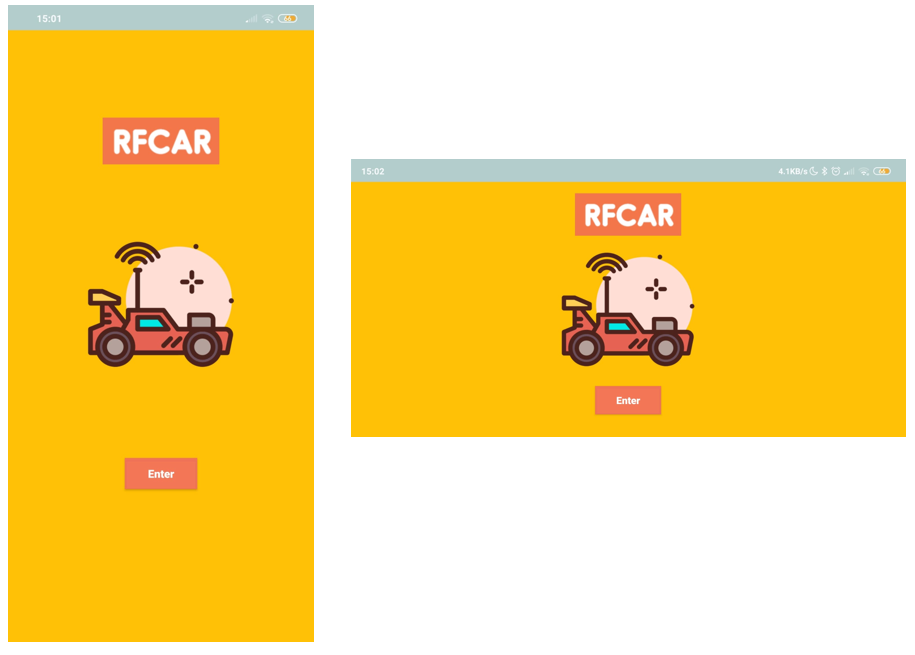
\includegraphics[width=0.8\textwidth]{img/orientation-test.png}
\caption{\label{fig:orientation-test}UI orientation test example}
\end{figure}
%%% Local Variables:
%%% mode: latex
%%% TeX-master: "../../../dissertation"
%%% End: